\documentclass[11pt,reqno]{amsart}
\usepackage{amssymb}
\usepackage[utf8]{inputenc}
\usepackage{tikz}
\usetikzlibrary{arrows.meta}
\usetikzlibrary{shapes.geometric}
\usetikzlibrary{patterns}
\usetikzlibrary{calc,scopes}
\usetikzlibrary{backgrounds}

\begin{document}

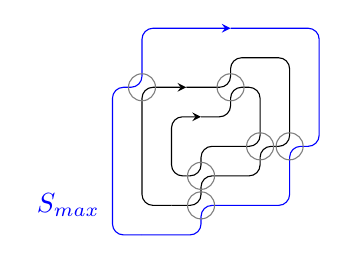
\begin{tikzpicture}[>=stealth,scale=3.75]
	\draw [rounded corners, blue, ->] (0.1,0)--(0,0)--(0,0.5)--(0.1,0.5)--(0.1,0.7) -- (0.4,0.7);
    \draw [rounded corners, blue] (0.4,0.7)--(0.7,0.7)--(0.7,0.3)--(0.6,0.3)--(0.6,0.1)--(0.3,0.1)--(0.3,0)--(0.1,0);
	\draw [rounded corners, ->] (0.2,0.1) -- (0.1,0.1)--(0.1,0.5) -- (0.25,0.5);
    \draw [rounded corners] (0.25,0.5)--(0.4,0.5)--(0.4,0.6)--(0.6,0.6)--(0.6,0.3)--(0.5,0.3)--(0.5,0.2)--(0.3,0.2)--(0.3,0.1)--(0.2,0.1);
	\draw [rounded corners, ->] (0.25,0.2)--(0.2,0.2)--(0.2,0.4)--(0.3,0.4);
    \draw [rounded corners] (0.3,0.4)--(0.4,0.4)--(0.4,0.5)--(0.5,0.5)--(0.5,0.3)--(0.3,0.3)--(0.3,0.2)--(0.25,0.2);
	\draw [blue] (-0.15, 0.1) node {$S_{max}$};

    \draw[gray] (0.1,0.5) circle (1.3pt);
    \draw[gray] (0.3,0.2) circle (1.3pt);
    \draw[gray] (0.3,0.1) circle (1.3pt);
    \draw[gray] (0.4,0.5) circle (1.3pt);
    \draw[gray] (0.5,0.3) circle (1.3pt);
    \draw[gray] (0.6,0.3) circle (1.3pt);
	\end{tikzpicture}

\end{document}